\documentclass[12pt,UTF8]{ctexart}
\usepackage{ctex,amsmath,amssymb,geometry,fancyhdr,bm,amsfonts,mathtools,extarrows,graphicx,url,enumerate,xcolor,float,multicol,wasysym}
\usepackage{subfigure}
\allowdisplaybreaks[4]
% 加入中文支持
\newcommand\Set[2]{\left\{#1\ \middle\vert\ #2 \right\}}
\newcommand\Lim[0]{\lim\limits_{n\rightarrow\infty}}
\newcommand\LIM[2]{\lim\limits_{#1\rightarrow#2}}
\newcommand\Ser[1]{\sum_{n=#1}^\infty}
\newcommand{\SER}[2]{\sum_{#1=#2}^\infty}
\newcommand{\Int}[4]{\varint\nolimits_{#1}^{#2}#3\mathrm d#4}
\newcommand{\aIInt}[1]{\iint\limits_{#1}}
\newcommand{\IInt}[3]{\iint\limits_{#1}#2\mathrm d#3}
\newcommand{\varIInt}[4]{\iint\limits_{#1}#2\mathrm d#3\mathrm d#4}
\newcommand{\IIInt}[3]{\iiint\limits_{#1}#2\mathrm d#3}
\newcommand{\varIIInt}[5]{\iiint\limits_{#1}#2\mathrm d#3\mathrm d#4\mathrm d#5}
\newcommand{\LInt}[3]{\varint\nolimits_{#1}#2\mathrm d#3}
\newcommand{\LOInt}[3]{\varoint\nolimits_{#1}#2\mathrm d#3}
\newcommand{\LLInt}[4]{\varint\nolimits_{#1}\nolimits^{#2}#3\mathrm d#4}
\newcommand{\BLInt}[2]{\varint\nolimits_{#1}#2}
\newcommand{\varBLInt}[3]{\varint\nolimits_{#1}\nolimits^{#2}#3}
\newcommand{\BLOInt}[2]{\varoint\nolimits_{#1}#2}
\newcommand{\SIInt}[3]{\iint\limits_{#1}#2\mathrm d#3}
\newcommand{\md}[1]{\mathrm d#1}
\newcommand{\BSIInt}[2]{\iint\limits_{#1}#2}
\newcommand{\pp}[2]{\frac{\partial #1}{\partial #2}}
\newcommand{\ppx}[1]{\frac{\partial #1}{\partial x}}
\newcommand{\ppy}[1]{\frac{\partial #1}{\partial y}}
\newcommand{\ppz}[1]{\frac{\partial #1}{\partial z}}
\newcommand{\varppx}[1]{\frac{\partial}{\partial x} #1}
\newcommand{\varppy}[1]{\frac{\partial}{\partial y} #1}
\newcommand{\varppz}[1]{\frac{\partial}{\partial z} #1}
\newcommand{\BSOIInt}[2]{\oiint\limits_{#1}#2}
\newcommand{\me}[0]{\mathrm e}
\geometry{a4paper,scale=0.80}
\pagestyle{fancy}
\rhead{多元函数积分学(2)}
\lhead{基础习题课期末复习}
\chead{微积分B(2)}
\begin{document}
\setcounter{section}{6}
\section{专题:变量替换}
\noindent
\subsection{复习计划}
\begin{figure}[H]
\begin{center}
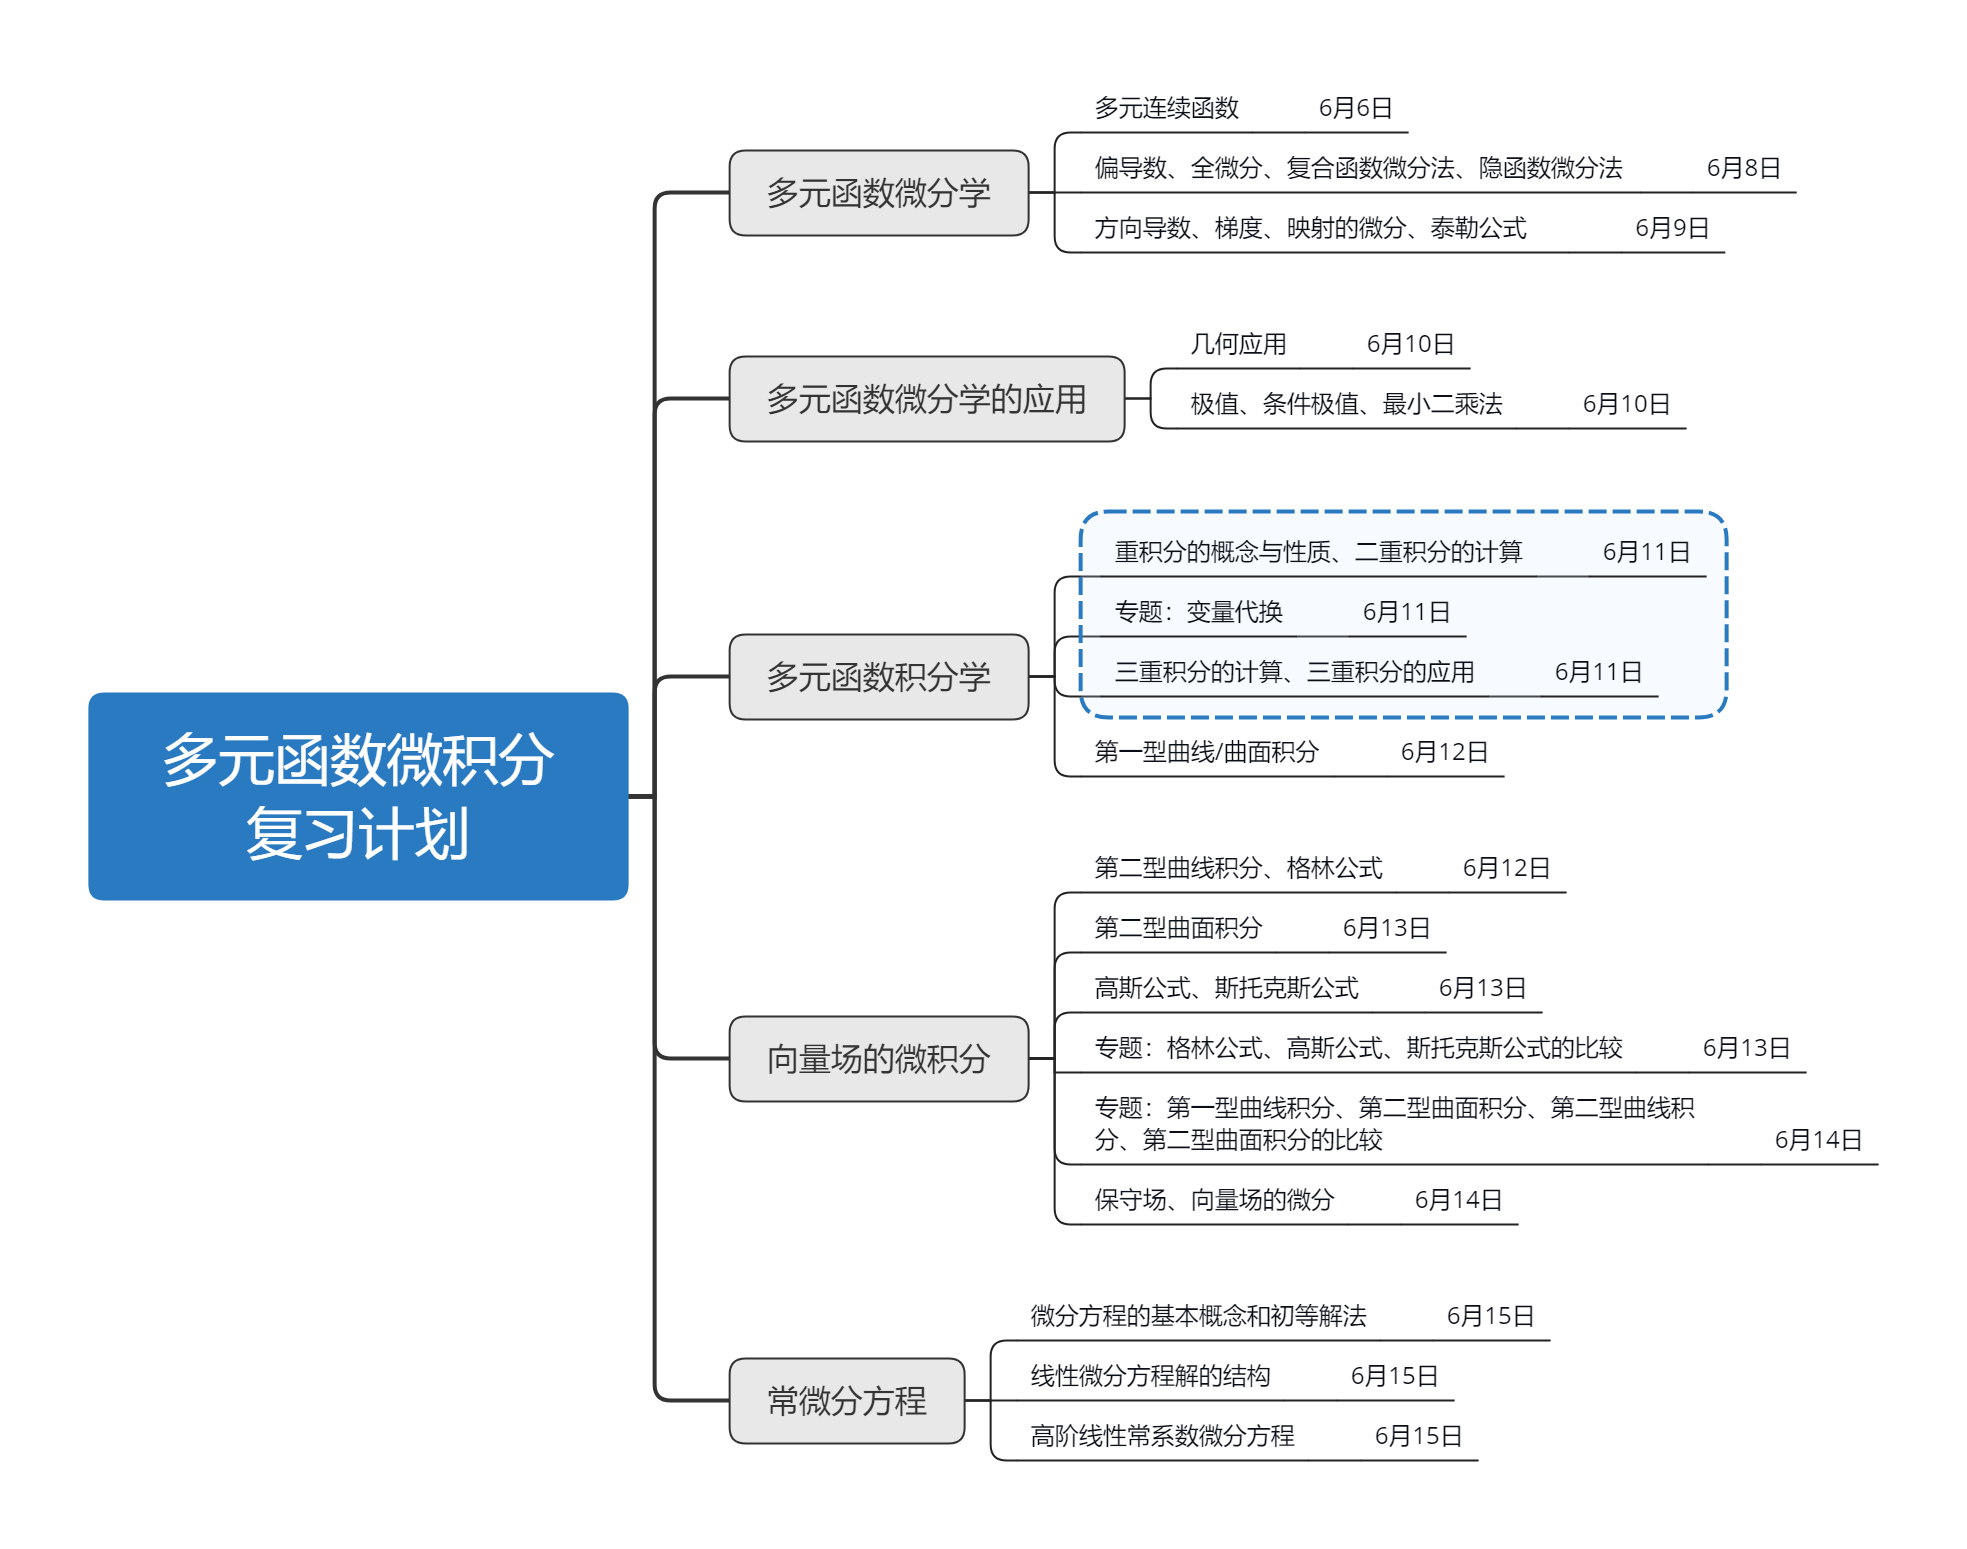
\includegraphics[height=0.5\textheight]{Figures20190611/plan.png}
\end{center}
\end{figure}
\subsection{习题分类与解题思路}
\begin{enumerate}
\item二重积分的变量替换公式:
\[
\iint_Df(x,y)\mathrm dx\mathrm dy=\iint_Df(x(u,v),y(u,v))|\frac{\mathrm D(x,y)}{\mathrm D(u,v)}|\mathrm du\mathrm dv=\iint_Df(x(u,v),y(u,v))\frac1{|\frac{\mathrm D(u,v)}{\mathrm D(x,y)}|}\mathrm du\mathrm dv.
\]
\item三重积分的变量替换公式:
\[\begin{aligned}
\iint_\Omega f(x,y,z)\mathrm dx\mathrm dy\mathrm dz&=\iint_\Omega f(x(u,v,w),y(u,v,w),z(u,v,w))|\frac{\mathrm D(x,y,z)}{\mathrm D(u,v,w)}|\mathrm du\mathrm dv\\
&=\iint_\Omega f(x(u,v,w),y(u,v,w),z(u,v,w))\frac1{|\frac{\mathrm D(u,v,w)}{\mathrm D(x,y,z)}|}\mathrm du\mathrm dv.
\end{aligned}\]
\item变量替换的目的:
\begin{enumerate}
\item使积分域更简单;
\item使被积函数更简单.
\end{enumerate}
\item变量替换主要有以下几种形式:
\begin{enumerate}
\item已知$y=kx$,可令$u=\frac yx$;
\item已知$xy=k$,可令$u=xy$;
\item已知$x+y=k$,可令$x+y=u$;
\item已知$x-y=k$,可令$x-y=u$;
\item已知$x^n+y^n=k$,可令$\begin{cases}x=r^{\frac1n}\cos^{\frac2n}\theta,\\ y=r^{\frac1n}\sin^{\frac2n}\theta.\end{cases}$
\end{enumerate}
\item解题思路:
\begin{enumerate}
\item[第一步]做变量代换,将积分域用新变量表示;
\item[第二步]求解雅可比行列式;
\item[第三步]利用变量替换公式计算重积分.
\end{enumerate}
\item以下是本章变量替换的习题汇总.
\end{enumerate}
\subsection{习题12.3解答}
\begin{enumerate}
\item求由$xy=a^2,xy=2a^2,y=x,y=2x$围成的第一象限区域的面积.

解:令$\begin{cases}
u=xy,\\
v=\frac yx,
\end{cases}$所求区域$D=\Set{(u,v)}{a^2\leqslant u\leqslant2a^2,1\leqslant v\leqslant2}$,

$\frac{\mathrm D(u,v)}{\mathrm D(x,y)}=\begin{vmatrix}
y&x\\
-\frac y{x^2}&\frac1x
\end{vmatrix}=\frac yx+\frac yx=2v,\ |\frac{\mathrm D(x,y)}{\mathrm D(u,v)}|=\frac1{2v}$,

所求面积$S=\IInt D{}\sigma=\varIInt D{|\frac{\mathrm D(x,y)}{\mathrm D(u,v)}|}uv=\Int{a^2}{2a^2}{}u\Int12{\frac1{2v}}v=a^2\frac12\ln v\big|_1^2=\frac{\ln2}2a^2$.

\item计算$I=\IInt D{\cos(\frac{x-y}{x+y})}\sigma,D$由$x+y=1,x=0,y=0$围成.

解:方法1:$\because$区域$D$关于$y=x$对称,且在关于$y=x$的对称点$(x,y)$和$(y,x)$处$\cos(\frac{x-y}{x+y})=\cos(\frac{y-x}{y+x})$,

$\therefore I=\IInt D{\cos(\frac{x-y}{x+y})}\sigma=2\IInt{D_1}{\cos(\frac{x-y}{x+y})}\sigma$,其中区域$D_1$由$x+y=1,y=0,y=x$围成.

令$\begin{cases}
u=x+y,\\
v=\frac yx,
\end{cases}$则$\begin{cases}
x=\frac u{1+v},\\
y=\frac{uv}{1+v},
\end{cases}$区域$D_1=\Set{(u,v)}{0\leqslant u\leqslant1,0\leqslant v\leqslant1}$,

$\frac{\mathrm D(u,v)}{\mathrm D(x,y)}=\begin{vmatrix}
1&1\\
-\frac y{x^2}&\frac1x
\end{vmatrix}=\frac{x+y}{x^2}=\frac{(1+v)^2}u,\ |\frac{\mathrm D(u,v)}{\mathrm D(x,y)}|=\frac u{(1+v)^2}$,

$\therefore I=2\IInt{D_1}{\cos(\frac{x-y}{x+y})}\sigma=2\varIInt{D_1}{\cos(\frac{1-v}{1+v})\frac u{(1+v)^2}}uv=2\Int01{\cos(\frac{1-v}{1+v})\frac1{(1+v)^2}}v\Int01uu\\
=\Int01{\cos(\frac{1-v}{1+v})\frac1{(1+v)^2}}v=\Int01{\cos(-1+\frac2{1+v})\frac1{(1+v)^2}}v=-\frac12\Int01{\cos(-1+\frac2{1+v})}{(-1+\frac2{1+v})}\\
=-\frac12\sin(-1+\frac2{1+v})\big|_0^1=\frac12\sin1$.

{\bf注}:如图\ref{12-3-2-1}所示.
\begin{figure}[H]
\begin{center}
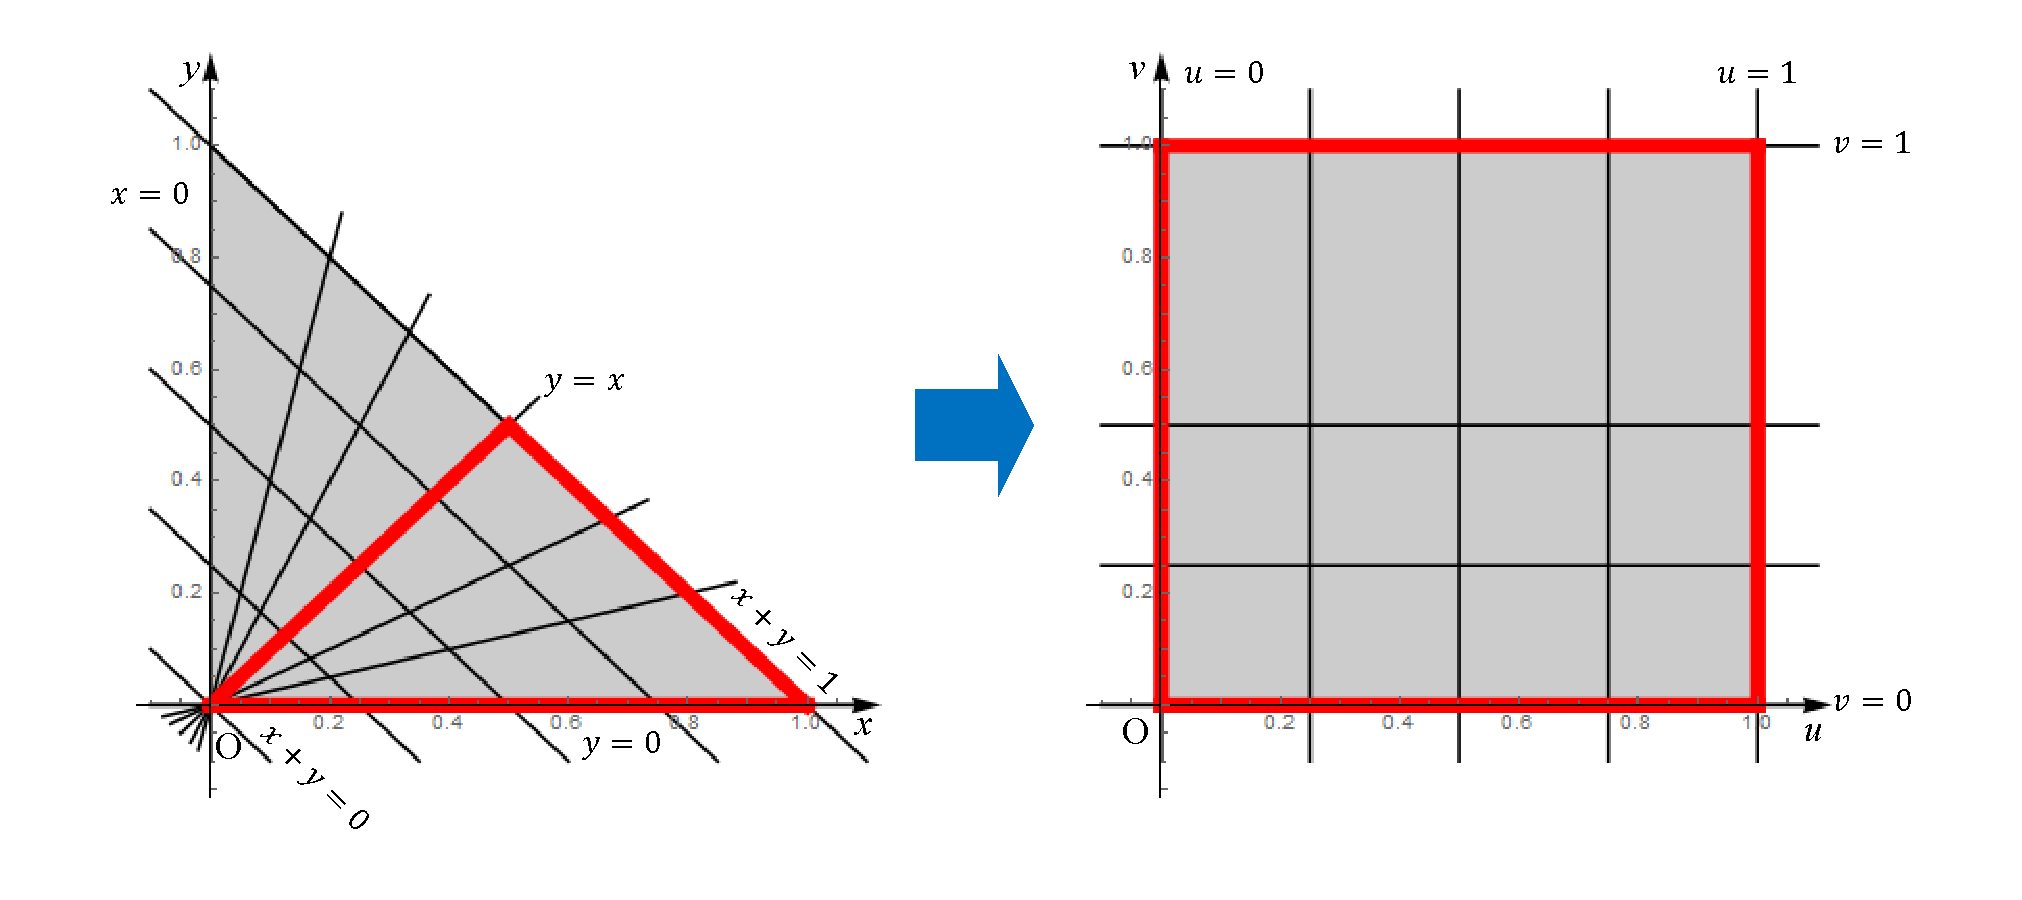
\includegraphics[height=0.3\textheight]{Figures/Fig12-3-2-1.pdf}
\end{center}
\caption{习题12.3 2题方法1图示}
\label{12-3-2-1}
\end{figure}

方法2:令$\begin{cases}
x=r\cos^2\theta,\\
y=r\sin^2\theta,
\end{cases}$则区域$D=\Set{(x,y)}{0\leqslant r\leqslant1,0\leqslant\theta\leqslant\frac\pi2}$,

$\frac{\mathrm D(x,y)}{\mathrm D(u,v)}=\begin{vmatrix}
\cos^2\theta&-2r\cos\theta\sin\theta\\
\sin^2\theta&2r\sin\theta\cos\theta
\end{vmatrix}=2r\sin\theta\cos^3\theta+2r\sin^3\theta\cos\theta=2r\sin\theta\cos\theta=r\sin2\theta$,

$\therefore I=\varIInt D{\cos(\frac{r\cos^2\theta-r\sin^2\theta}{r\cos^2\theta+r\sin^2\theta})|\frac{\mathrm D(x,y)}{\mathrm D(u,v)}|}r\theta=\varIInt D{\cos(\cos2\theta)r\sin2\theta}r\theta=\Int0{\frac\pi2}{\cos(\cos2\theta)\sin2\theta}\theta\Int01rr\\
=-\frac12\Int0{\frac\pi2}{\cos(\cos2\theta)}{\cos2\theta}\Int01rr=-\frac12\sin(\cos2\theta)\big|_0^{\frac\pi2}\frac12r^2\big|_0^1=-\frac12[\sin(-1)-\sin1]\frac12\\
=\frac12\sin1$.

{\bf注}:如图\ref{12-3-2-2}所示.
\begin{figure}[H]
\begin{center}
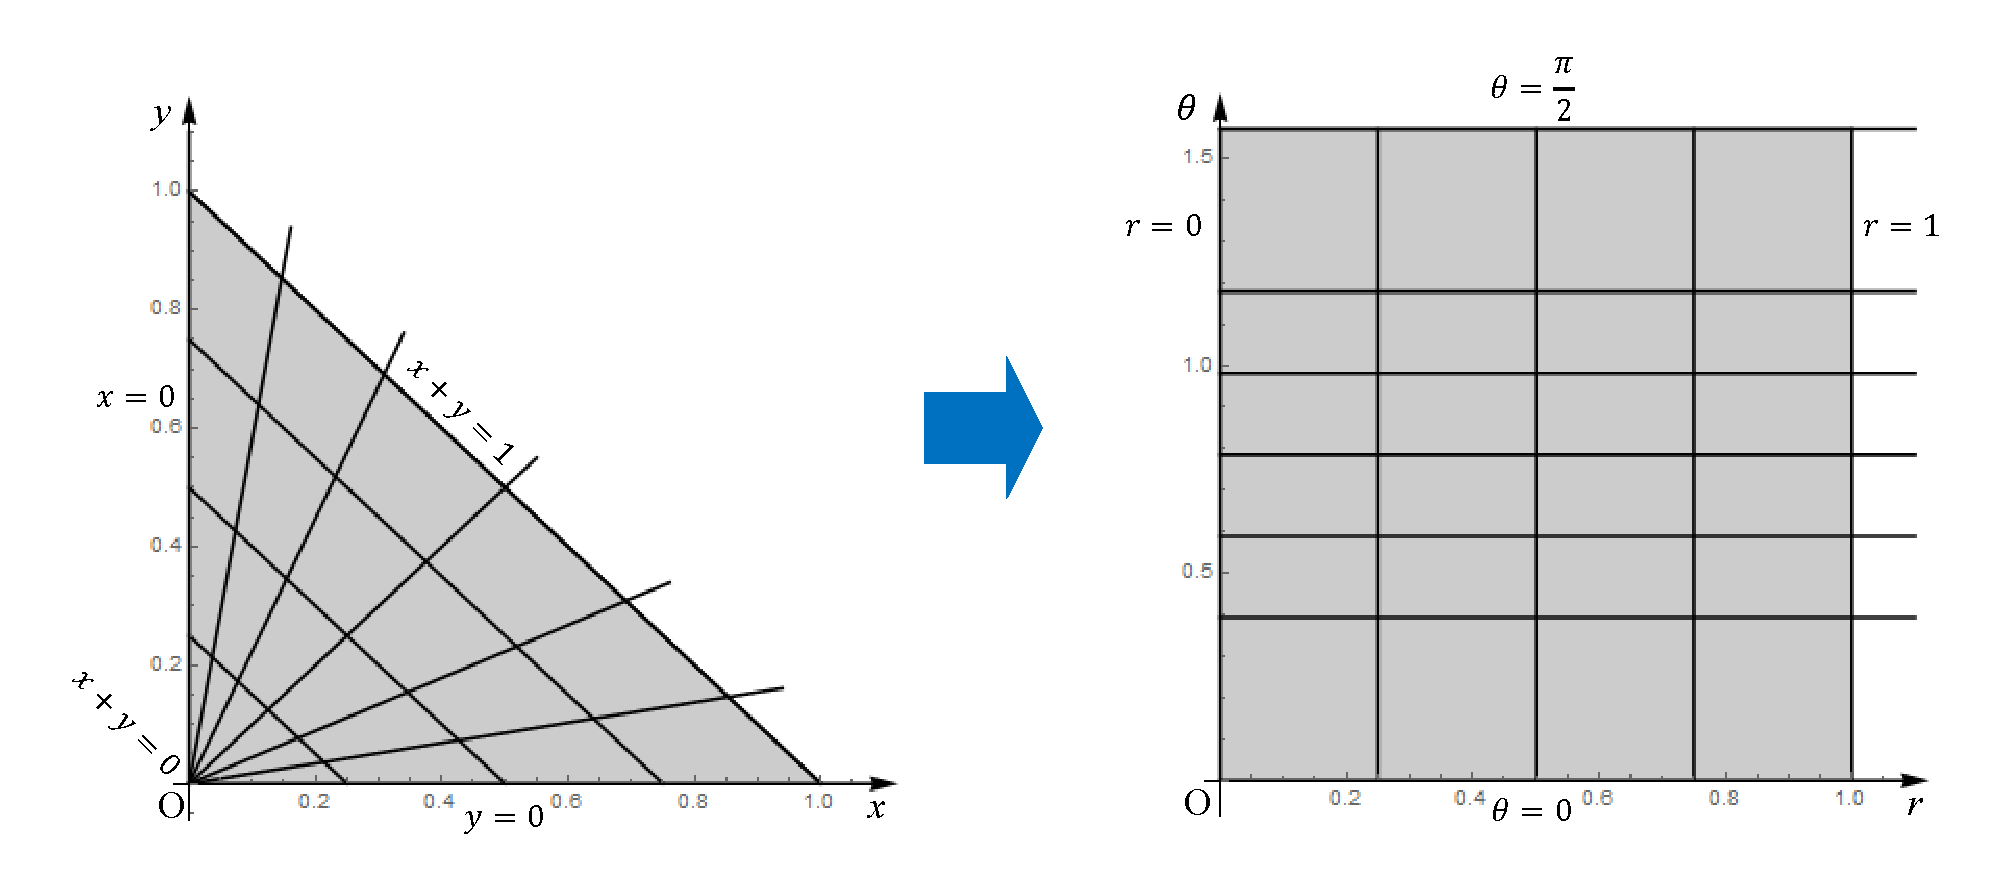
\includegraphics[height=0.3\textheight]{Figures/Fig12-3-2-2.pdf}
\end{center}
\caption{习题12.3 2题方法2图示}
\label{12-3-2-2}
\end{figure}

方法3:令$\begin{cases}
u=x-y,\\
v=x+y,
\end{cases}$则令$\begin{cases}
x=\frac12(u+v),\\
y=\frac12(v-u),
\end{cases}$区域$D=\Set{(u,v)}{0\leqslant v\leqslant1,-v\leqslant u\leqslant v}$,

$\frac{\mathrm D(x,y)}{\mathrm D(u,v)}=\begin{vmatrix}
\frac12&\frac12\\
-\frac12&\frac12
\end{vmatrix}=\frac12$,

$\therefore I=\varIInt D{\cos(\frac uv)|\frac{\mathrm D(x,y)}{\mathrm D(u,v)}|}uv=\frac12\varIInt D{\cos(\frac uv)}uv=\frac12\Int01{}v\Int{-v}v{\cos(\frac uv)}u=\frac12\Int01{}v\Int{-v}v{v\cos(\frac uv)}{\frac uv}\\
=\frac12\Int01{}v[v\sin(\frac uv)]_{-v}^v=\frac12\Int01{[v\sin1-v\sin(-1)]}v=\sin1\Int01vv=\frac12\sin1$.

注意:因为被积函数是$\cos(\frac uv)$,该函数无关于$v$初等原函数,故这种变量代换的方法应先积$u$后积$v$.

{\bf注}:如图\ref{12-3-2-3}所示.
\begin{figure}[H]
\begin{center}
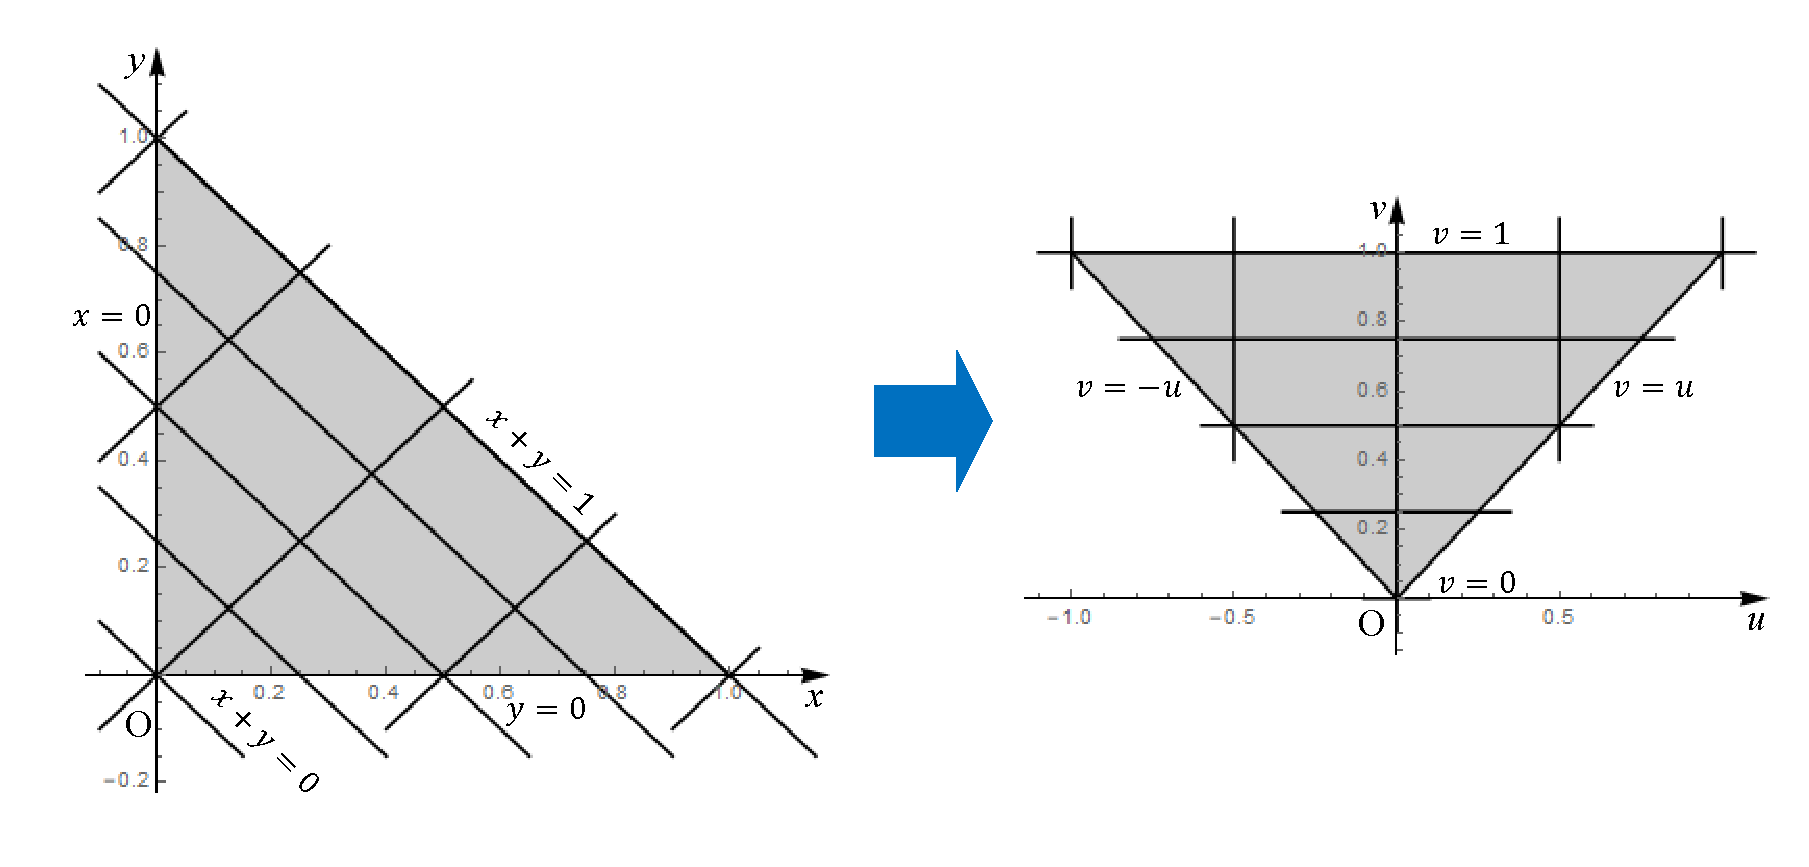
\includegraphics[height=0.3\textheight]{Figures/Fig12-3-2-3.pdf}
\end{center}
\caption{习题12.3 2题方法3图示}
\label{12-3-2-3}
\end{figure}

\item计算$I=\IInt D{(\sqrt x+\sqrt y)}\sigma,D=\Set{(x,y)}{\sqrt x+\sqrt y\leqslant1}$.

解:方法1:令$\begin{cases}
x=r^2\cos^4\theta,\\
y=r^2\sin^4\theta,
\end{cases}$则区域$D=\Set{(r,\theta)}{0\leqslant r\leqslant1,0\leqslant\theta\leqslant\frac\pi2}$,

$\frac{\mathrm D(x,y)}{\mathrm D(r,\theta)}=\begin{vmatrix}
2r\cos^4\theta&-4r^2\cos^3\theta\sin\theta\\
2r\sin^4\theta&4r^2\sin^3\theta\cos\theta
\end{vmatrix}=8r^3\sin^3\theta\cos^3\theta$,

$\therefore I=\IInt D{(\sqrt x+\sqrt y)}\sigma=\varIInt D{r|\frac{\mathrm D(x,y)}{\mathrm D(r,\theta)}|}uv=\varIInt D{8r^4\sin^3\theta\cos^3\theta}uv=\Int01{r^4}r\Int0{\frac\pi2}{2^3\sin^3\theta\cos^3\theta}\theta\\
=\frac15r^5\big|_0^1\frac12\Int0{\frac\pi2}{\sin^32\theta}{2\theta}=\frac1{10}\Int0{\frac\pi2}{\sin^32\theta}{2\theta}=\frac1{10}\Int0\pi{\sin^3\varphi}\varphi=\frac2{10}\Int0{\frac\pi2}{\sin^3\varphi}\varphi=\frac15\frac{2}{3}=\frac2{15}$.

方法2:令$\begin{cases}
u=\sqrt x,\\
v=\sqrt y,
\end{cases}$则$\begin{cases}
x=u^2,\\
y=v^2,
\end{cases}$区域$D=\Set{(u,v)}{0\leqslant u\leqslant1,0\leqslant v\leqslant1-u}$,

$\frac{\mathrm D(x,y)}{\mathrm D(u,v)}=\begin{vmatrix}
2u&0\\
0&2v
\end{vmatrix}=4uv$,

$\therefore I=\IInt D{(\sqrt x+\sqrt y)}\sigma=\varIInt D{(u+v)|\frac{\mathrm D(x,y)}{\mathrm D(u,v)}|}uv=\varIInt D{(u+v)4uv}uv\\
=4\Int01{}u\Int0{1-u}{(u^2v+uv^2)}v=4\Int01{(\frac12u^2v^2+\frac13uv^3)\big|_0^{1-u}}u\\
=4\Int01{[\frac12u^2(1-u)^2+\frac13u(1-u)^3]}u=4\Int01{(\frac12u^2-u^3+\frac12u^4+\frac13u-u^2+u^3-\frac13u^4)}u\\
=4\Int01{(-\frac12u^2+\frac16u^4+\frac13u)}u=4(-\frac16u^3+\frac1{30}u^5+\frac16u^2)\big|_0^1=\frac2{15}$.

\item在第1象限中,设$D$由$xy=1,xy=2,\frac yx=1$及$\frac yx=4$围成,试证:
\[
\IInt D{f(xy)}\sigma=\ln2\Int12{f(x)}x.
\]
证明:令$\begin{cases}
u=xy,\\
v=\frac yx,
\end{cases}$则区域$D=\Set{(u,v)}{1\leqslant u\leqslant2,1\leqslant v\leqslant4}$,

$\frac{\mathrm D(u,v)}{\mathrm D(x,y)}=\begin{vmatrix}
y&x\\
-\frac y{x^2}&\frac1x
\end{vmatrix}=\frac yx+\frac yx=2v,\ |\frac{\mathrm D(x,y)}{\mathrm D(u,v)}|=\frac1{2v}$,

$\therefore\IInt D{f(xy)}\sigma=\varIInt D{f(u)|\frac{\mathrm D(x,y)}{\mathrm D(u,v)}|}uv=\Int12{f(u)}u\Int14{\frac1{2v}}v=\frac12\ln v\big|_1^4\Int12{f(u)}u\\
=2\ln2\Int12{f(u)}u=\ln2\Int12{f(x)}x.$
\end{enumerate}
\subsection{习题12.4解答}
\begin{enumerate}
\item[15]求由平面$a_1x+b_1y+c_1z=\pm h_1,a_2x+b_2y+c_2z=\pm h_2,a_3x+b_3y+c_3z=\pm h_3$所围成平行六面体的体积.

解:令$\begin{cases}
u=a_1x+b_1y+c_1z,\\
v=a_2x+b_2y+c_2z,\\
w=a_3x+b_3y+c_3z,
\end{cases}$不妨设$h_1>0,h_2>0,h_3>0$,则该平行六面体可表示为$\Omega=\Set{(u,v,w)}{-h_1\leqslant u\leqslant h_1,-h_2\leqslant v\leqslant h_2,-h_3\leqslant w\leqslant h_3}$,

$\frac{\mathrm D(u,v,w)}{\mathrm D(x,y,z)}=\begin{vmatrix}
a_1&b_1&c_1\\
a_2&b_2&c_2\\
a_3&b_3&c_3
\end{vmatrix}=\det A$,

当$\det A\neq0$时,\\
$\varIIInt\Omega{}xyz=\varIIInt\Omega{|\frac{\mathrm D(x,y,z)}{\mathrm D(u,v,w)}|}uvw=\varIIInt\Omega{\frac1{|\frac{\mathrm D(u,v,w)}{\mathrm D(x,y,z)}|}}uvw=\varIIInt\Omega{\frac1{|\det A|}}uvw\\
=\frac1{|\det A|}\varIIInt\Omega{}uvw=\frac{2h_1\cdot2h_2\cdot2h_3}{|\det A|}=\frac{8h_1h_2h_3}{|\det A|}$.

\end{enumerate}
\subsection{第12章补充题解答}
\begin{enumerate}
\item[8]设$D=\Set{(x,y)}{|x|+|y|\leqslant1}$,将$\varIInt D{f(x+y)}xy$化为定积分.

\begin{figure}[H]
\begin{center}
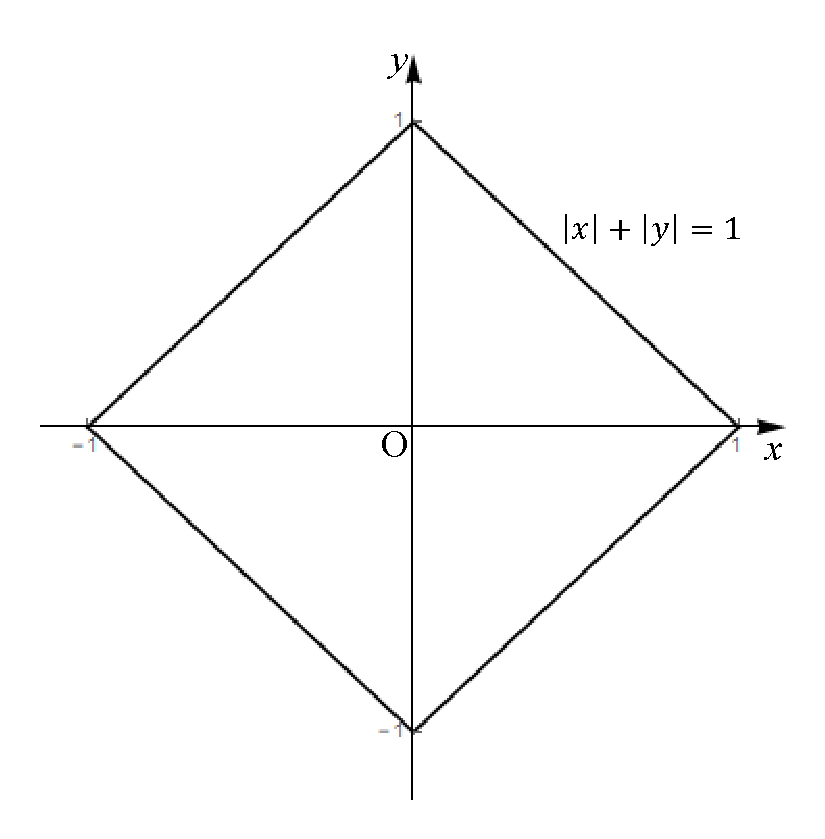
\includegraphics[height=0.3\textheight]{Figures21/Fig12-C-8.pdf}
\end{center}
\caption{第12章补充题 8.题图示}
\label{12-C-8}
\end{figure}

解:方法1:令$\begin{cases}
u=x+y,\\
v=x-y,
\end{cases}$则$D=\Set{(u,v)}{-1\leqslant u\leqslant 1,-1\leqslant v\leqslant 1}$,

$\frac{\mathrm D(u,v)}{\mathrm D(x,y)}=\begin{vmatrix}
1&1\\
1&-1
\end{vmatrix}=-2$,

$\therefore\varIInt D{f(x+y)}xy=\varIInt D{f(u)\frac1{|\frac{\mathrm D(u,v)}{\mathrm D(x,y)}|}}uv=\varIInt D{\frac12f(u)}uv=\frac12\Int{-1}1{}v\Int{-1}1{f(u)}u\\
=\Int{-1}1{f(u)}u$.

方法2:将重积分化为累次积分,有
\[
\varIInt{|x|+|y|\leqslant1}{f(x+y)}xy=\Int{-1}0{}x\Int{-1-x}{1+x}{f(x+y)}y+\Int01{}x\Int{-1+x}{1-x}{f(x+y)}y,
\]
令$x+y=u$,
\[\begin{split}
\text{上式}&=\Int{-1}0{}x\Int{-1}{1+2x}{f(u)}u+\Int01{x}\Int{2x-1}1{f(u)}u\\
&=\Int{-1}1{f(u)}u\Int{\frac{u-1}2}{\frac{u+1}2}{}x=\Int{-1}1{f(u)}u.
\end{split}\]
\item[10]计算下列积分:\\
(1)$\IIInt\Omega{(ax+by+cz)^2}V$,其中$\Omega=\Set{(x,y,z)}{x^2+y^2+z^2\leqslant R^2}$;\\
(2)$\IIInt\Omega{(\frac{x^2}{a^2}+\frac{y^2}{b^2}+\frac{z^2}{c^2})}V$,其中$\Omega=\Set{(x,y,z)}{\frac{x^2}{a^2}+\frac{y^2}{b^2}+\frac{z^2}{c^2}\leqslant1}$.

解:(1)方法1:由对称性可知

$\IIInt\Omega{(ax+by+cz)^2}V=\IIInt\Omega{(a^2x^2+b^2y^2+c^2z^2+2abxy+2acxz+2bcyz)}V\\
=\IIInt\Omega{(a^2x^2+b^2y^2+c^2z^2)}V=(a^2+b^2+c^2)\IIInt\Omega{z^2}V\\
=(a^2+b^2+c^2)\varIIInt\Omega{r^2\cos^2\varphi\cdot r^2\sin\varphi}\theta\varphi r\\
=(a^2+b^2+c^2)\Int0{2\pi}{}\theta\Int0R{r^4}r\Int0\pi{\cos^2\varphi\sin\varphi}\varphi\\
=\frac25\pi R^4(a^2+b^2+c^2)(-\frac13\cos^3\varphi)\big|_0^\pi=\frac4{15}\pi R^4(a^2+b^2+c^2)$.

方法2:$\IIInt\Omega{(ax+by+cz)^2}V=\IIInt\Omega{(a^2x^2+b^2y^2+c^2z^2+2abxy+2acxz+2bcyz)}V\\
=\IIInt\Omega{(a^2x^2+b^2y^2+c^2z^2)}V=(a^2+b^2+c^2)\IIInt\Omega{z^2}V=\frac13(a^2+b^2+c^2)\IIInt\Omega{(x^2+y^2+z^2)}V\\
=\frac13(a^2+b^2+c^2)\Int0{2\pi}{}\theta\Int0\pi{}\varphi\Int0R{r^2\cdot r^2\sin\varphi}r=\frac23\pi(a^2+b^2+c^2)\Int0\pi{\sin\varphi}\varphi\Int0R{r^4}r\\
=\frac23\pi(a^2+b^2+c^2)(-\cos\varphi)\big|_0^\pi\frac15r^5\big|_0^R=\frac4{15}\pi R^4(a^2+b^2+c^2)$.

(2)令$\begin{cases}
x=au,\\
y=bv,\\
z=cw,
\end{cases}$则$\Omega=\Set{(u,v,w)}{u^2+v^2+w^2\leqslant1}$,

$\frac{\mathrm D(x,y,z)}{\mathrm D(u,v,w)}=\begin{vmatrix}
a&0&0\\
0&b&0\\
0&0&c
\end{vmatrix}=abc$,

$\therefore\IIInt\Omega{(\frac{x^2}{a^2}+\frac{y^2}{b^2}+\frac{z^2}{c^2})}V=\varIIInt\Omega{(u^2+v^2+w^2)|\frac{\mathrm D(u,v,w)}{\mathrm D(x,y,z)}|}uvw=abc\varIIInt\Omega{(u^2+v^2+w^2)}uvw\\
=abc\frac4{15}\pi 1^4(1^2+1^2+1^2)=\frac45\pi abc$.

\end{enumerate}
\end{document}